\begin{problem}%
{Творческие личности}%
{\textsl{стандартный ввод}}%
{\textsl{стандартный вывод}}%
{1 секунда}%
{256 мегабайт}%
{}

Молодой известный дизайнер Пётр решил устроить мастер-класс для широких масс. Он планирует, что на мастер-классе каждый участник создаст свой неповторимый шедевр. Пётр собирается подготовить для каждого участника огромный белый холст $h$ см $\times$ $w$ см  ($h$ и $m$ — целые числа) и баночку краски чёрного цвета, которой хватает ровно на $s$ см\textsuperscript{2}  холста.\\

Незадолго до мастер-класса Петру сообщили, что широкие массы не блещут оригинальностью, и каждый участник нарисует ровно один прямоугольник, истратив при этом целиком свою баночку краски. Более того, стороны прямоугольника обязательно будут параллельны осям холста, а расстояния от сторон прямоугольника до сторон холста будут выражаться целыми числами сантиметров. Пётр заинтересовался, сколько можно нарисовать различных произведений искусства (банальных, но всё же примечательных!) в данных условиях?

\InputFile

В одной строке заданы три целых числа $h$, $w$, $s$ ($1 \le h, w \le 10^5$, $1 \le s \le 10^9$) — размеры холста и площадь прямоугольника.

\OutputFile

Выведите одно целое число — ответ на задачу.

\Examples

\begin{example}
\exmp{
4 2 4
}{%
5
}%
\exmp{
3 2 2
}{%
7
}%
\exmp{
2 3 10
}{%
0
}%
\end{example}

\Explanation

В первом примере из условия есть два вида прямоугольников с площадью $4$ см\textsuperscript{2}. Прямоугольник $1$ см $\times$ $4$ см можно разместить двумя способами, а прямоугольник $2$ см $\times$ $2$ см — тремя способами.

\begin{center}
\begin{adjustbox}{max size={\textwidth}{\textheight}}
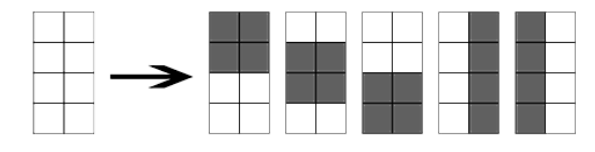
\includegraphics{images/2964.png}
\end{adjustbox}
\end{center}

Во втором примере из условия есть два вида прямоугольников с площадью $2$ см\textsuperscript{2}. Прямоугольник $1$ см $\times$ $2$ см  можно разместить четырьмя способами, а прямоугольник $2$ см $\times$ $1$ см  — тремя способами.

\begin{center}
\begin{adjustbox}{max size={\textwidth}{\textheight}}
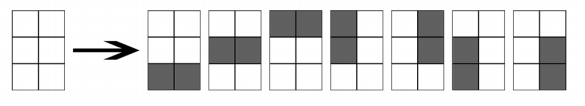
\includegraphics{images/2965.png}
\end{adjustbox}
\end{center}

В третьем примере из условия площадь холста слишком мала для столь большого количества краски, поэтому нарисовать произведение искусства в таких условиях невозможно.

\end{problem}